%% ============================================================
%%  chapter03_slides.tex
%%  New Exact Algorithms for the Capacitated Vehicle Routing Problem
%%  Vehicle Routing: Problems, Methods, and Applications, 2nd ed., 2014
%%  Authors covered: Marcus Poggi & Eduardo Uchoa
%% ============================================================
\documentclass[aspectratio=169,10pt]{beamer}

\usetheme{Madrid}
\usecolortheme{seahorse}
\setbeamertemplate{footline}[frame number]
\setbeamertemplate{navigation symbols}{}

\usepackage{amsmath,amssymb,amsfonts}
\usepackage{mathtools}
\usepackage{booktabs}
\usepackage{array}
\usepackage{graphicx}
\usepackage{xcolor}
\usepackage{listings}
\usepackage{tikz}
\usetikzlibrary{arrows.meta,shapes,positioning,fit,calc}
\usepackage{algorithm}
\usepackage{algpseudocode}
\usepackage{multirow}
\usepackage{tabularx}
\usepackage{hyperref}

\graphicspath{{figures/}}

\lstset{
  language=Python,
  basicstyle=\ttfamily\scriptsize,
  numbers=left,
  numberstyle=\tiny\color{gray},
  frame=single,
  backgroundcolor=\color{gray!7},
  commentstyle=\color{green!50!black}\itshape,
  keywordstyle=\color{blue}\bfseries,
  stringstyle=\color{orange!80!black},
  breaklines=true,
  showstringspaces=false,
  tabsize=4,
}

%% ---- colour shortcuts -----
\definecolor{depotblue}{RGB}{30,80,160}
\definecolor{cutred}{RGB}{190,30,30}
\definecolor{pricinggreen}{RGB}{20,130,60}

%% ============================================================
\title[New Exact Algorithms -- CVRP]{%
  New Exact Algorithms\\for the Capacitated Vehicle Routing Problem}
\subtitle{Chapter 3 --- Vehicle Routing: Problems, Methods,
          and Applications, 2nd Edition (2014)}
\author{Marcus Poggi \and Eduardo Uchoa}
\institute{Pontifical Catholic University of Rio de Janeiro (PUC-Rio)}
\date{Slides prepared for self-study, 2024}
%% ============================================================

\begin{document}

\begin{frame}
  \titlepage
\end{frame}

%% ---- TOC ---------------------------------------------------
\begin{frame}[allowframebreaks]{Table of Contents}
  \tableofcontents
\end{frame}

%% ============================================================
\section{Introduction}
%% ============================================================

\begin{frame}[allowframebreaks]{Introduction}

The Capacitated Vehicle Routing Problem (CVRP) is one of the most
intensely studied combinatorial optimisation problems. Given a depot,
a set of customers each with a known demand, a homogeneous fleet of
vehicles each with capacity $Q$, the goal is to design a minimum-cost
set of routes such that every customer is visited exactly once, each
route starts and ends at the depot, and no route exceeds the vehicle
capacity.

\begin{block}{Why exact methods matter}
Heuristics can find good solutions quickly, but exact methods prove
optimality and establish tight lower bounds. These bounds are crucial
for benchmarking heuristics and understanding the hardness of specific
instances. Since the seminal work of Dantzig, Ramser, and Dantzig (1959),
generation of exact algorithms has been the dominant approach for building
Branch-and-Cut and Branch-Price-Cut (BPC) solvers.
\end{block}

\framebreak

The chapter surveys the most recent (circa 2012--2014) exact approaches
for the CVRP. The key insight is that \emph{column generation} combined
with \emph{cutting planes} and \emph{branching} yields solvers that can
handle instances with up to 200 customers --- roughly an order of magnitude
larger than what was possible a decade earlier.

Three families of algorithms are reviewed in detail:
\begin{enumerate}
  \item \textbf{Fukasawa et al.\ \cite{Fuk06}} --- BPC algorithm with the
        following features:
        \begin{itemize}
          \item Based on the elementary states that allow multiple visits to
                the same customer in the LP relaxation.
          \item Includes the two-commodity VRP formulation.
          \item A column-generation subroutine to add new routes.
        \end{itemize}
  \item \textbf{Baldacci, Mingozzi, and Marchetti} --- presenting an
        algorithm based on the column enumeration, which is initialised
        with an exact solving of the LP relaxation and MIP solver on top.
  \item \textbf{Contardo and Martinelli \cite{Con14}} --- improving BPC
        performance by introducing new cuts, better branching strategies,
        and aggressive heuristic strong-branching.
\end{enumerate}

\framebreak

\begin{alertblock}{Historical context}
In the early 1990s, instances with $n \approx 30$ customers were considered
large. By 2006 (Fukasawa et al.), instances up to $n \approx 100$ could be
solved. By 2014 (Contardo and Martinelli), the frontier had moved to
$n \approx 200$. The chapter documents this progress and highlights the
algorithmic innovations responsible for it.
\end{alertblock}

The chapter is structured around three main components of any BPC algorithm
for the CVRP: (1) the LP relaxation and its formulations,
(2) valid inequalities (cutting planes) that tighten the LP bound, and
(3) the pricing sub-problem that generates new columns during column generation.
Together these three components, plus a branching strategy, form a
state-of-the-art exact solver.

\end{frame}

%% ============================================================
\section{Main Exact Approaches}
%% ============================================================

\begin{frame}[allowframebreaks]{Overview of Branch-Price-Cut (BPC)}

The dominant paradigm for solving the CVRP exactly is
\emph{branch-and-price-and-cut} (BPC). This is an extension of the
classical branch-and-bound framework in which:
\begin{itemize}
  \item The LP relaxation at each node is solved by \emph{column generation}
        (pricing) rather than directly, because the number of feasible routes
        is exponential.
  \item \emph{Cutting planes} (valid inequalities) are added to strengthen
        the LP relaxation before and during branching.
  \item \emph{Branching} resolves fractional solutions until an integer
        (feasible) solution is obtained.
\end{itemize}

\begin{figure}
  \centering
  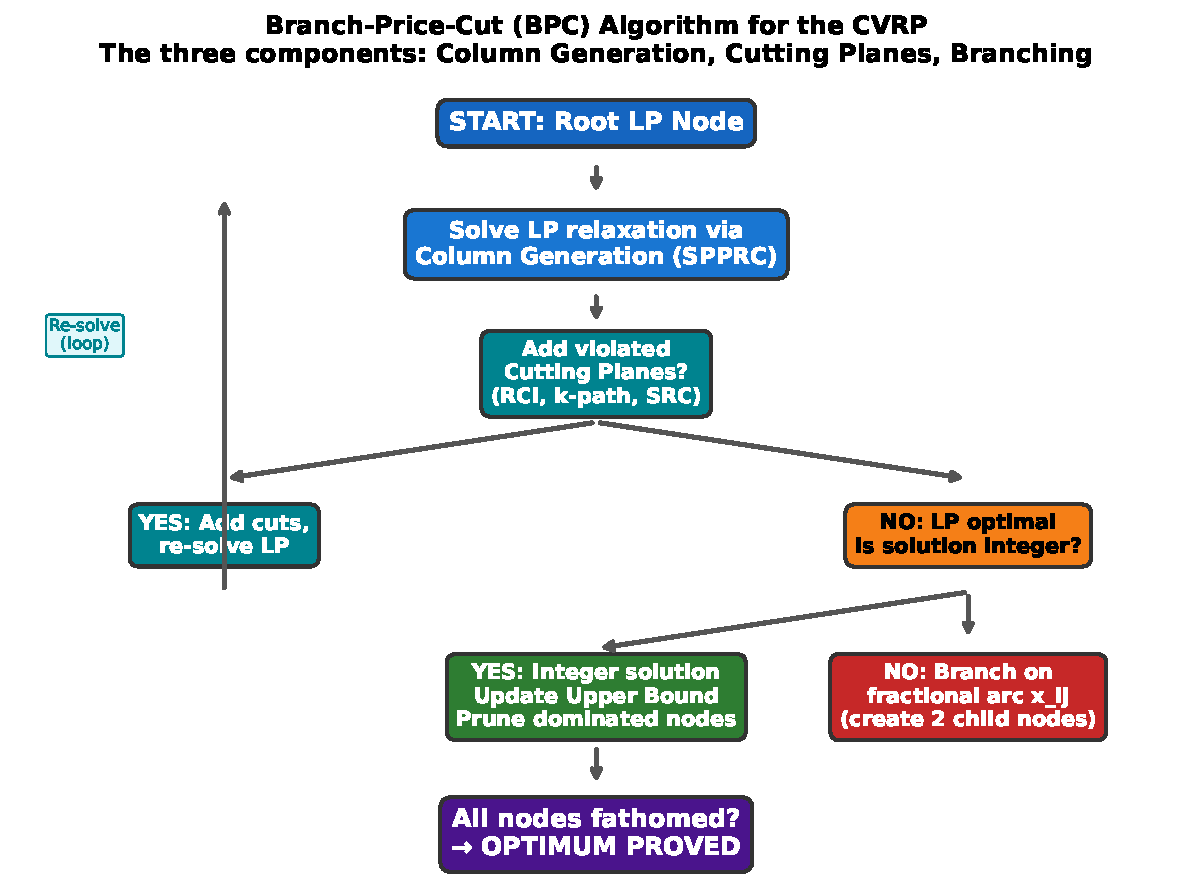
\includegraphics[width=0.72\linewidth]{fig_bpc_flowchart.pdf}
  \caption{Schematic flowchart of a Branch-Price-Cut algorithm for the CVRP.
           At each tree node the LP is solved by column generation, cuts are
           added if they separate the current fractional point, and then
           the solver branches on a fractional variable.}
\end{figure}

\framebreak

\begin{block}{The four pillars of BPC}
\begin{enumerate}
  \item \textbf{Formulation.} Choose a mathematical model whose LP relaxation
        gives a strong lower bound. The \emph{set-partitioning} (SP)
        formulation is preferred because it provides the best bound, but
        it has one variable per feasible route (exponentially many).
  \item \textbf{Column generation.} Solve the LP relaxation of the SP by
        starting with a small set of routes and iteratively adding the
        route with the most negative reduced cost. This requires solving
        a \emph{Shortest Path with Resource Constraints (SPPRC)} sub-problem.
  \item \textbf{Cutting planes.} Identify valid inequalities violated by the
        current LP solution and add them. Capacity cuts, $k$-path cuts, and
        Subset Row Cuts (SRC) are the most effective families.
  \item \textbf{Branching.} When no violated cut exists and the LP solution
        is fractional, branch on a fractional edge variable or on a flow
        variable to partition the search space.
\end{enumerate}
\end{block}

\framebreak

The figure below illustrates a small BPC tree. Each node stores the LP
lower bound (LB) for the sub-problem at that node; nodes whose LB exceeds
the best known integer solution (upper bound, UB) are pruned.

\begin{figure}
  \centering
  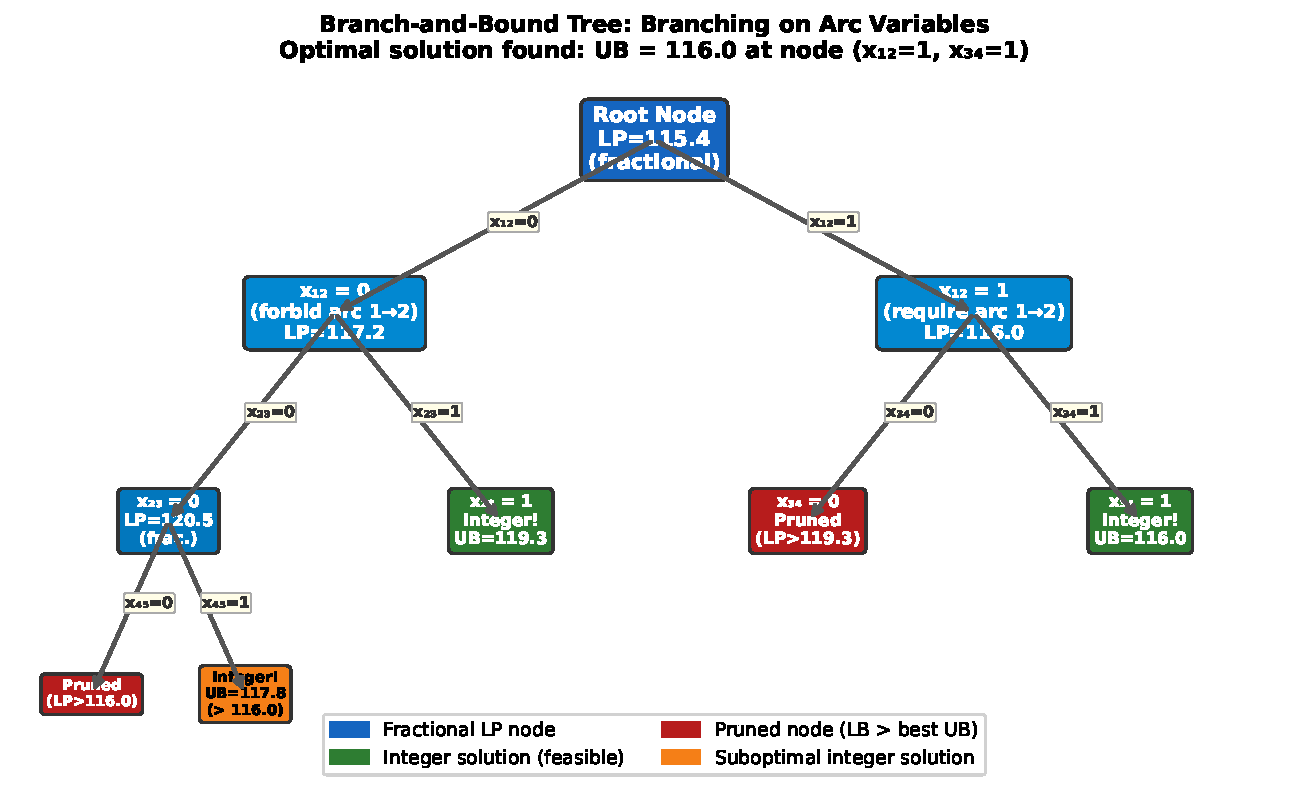
\includegraphics[width=0.68\linewidth]{fig_bb_tree.pdf}
  \caption{A schematic BPC tree. Leaves marked ``Feasible'' have integer LP
           solutions; leaves marked ``Pruned'' have LP bounds exceeding the
           current best upper bound. The tree is explored depth-first or
           best-first.}
\end{figure}

\end{frame}

%% ============================================================
\section{Formulations}
%% ============================================================

\begin{frame}[allowframebreaks]{The Two-Index Formulation}

The classical two-index formulation of the CVRP, also known as the
\emph{vehicle-flow} formulation, was introduced by Laporte, Nobert,
and Desrochers (1985).

\begin{block}{Two-Index VRP (2-index)}
Let $V = \{0, 1, \ldots, n\}$ where node 0 is the depot and nodes
$1, \ldots, n$ are customers. Let $A$ denote the set of directed arcs
$(i,j)$ for $i \neq j$. Define:
\begin{align*}
  x_{ij} &= \text{number of times arc } (i,j) \text{ is used by some vehicle}\\
  c_{ij} &= \text{travel cost of arc } (i,j)
\end{align*}

\begin{align}
  \text{(VRP)} \quad \min \quad & \sum_{(i,j)\in A} c_{ij}\, x_{ij} \tag{3.1}\\
  \text{s.t.} \quad
  & \sum_{j\in V} x_{ij} = 1 \quad \forall\, i \in V\setminus\{0\} \tag{3.2}\\
  & \sum_{j\in V} x_{ji} = 1 \quad \forall\, i \in V\setminus\{0\} \tag{3.3}\\
  & \sum_{j\in V} x_{0j} = K \tag{3.4}\\
  & x(\delta(S)) \geq 2\Big\lceil d(S)/Q \Big\rceil
    \quad \forall\, S \subseteq V\setminus\{0\},\, S \neq \emptyset \tag{3.5}\\
  & x_{ij} \in \{0, 1\} \quad \forall\, (i,j)\in A \tag{3.6}
\end{align}
\end{block}

\framebreak

Each symbol in the two-index formulation plays a distinct role. Constraints
(3.2) and (3.3) are degree constraints: they ensure that every customer is
entered exactly once and left exactly once. Constraint (3.4) fixes the
number of routes at $K$ (or enforces an upper bound if $K$ is a variable).
Constraint (3.5) is the \emph{capacity cut} (also called rounded capacity
inequalities, RCI): it says that the number of edges crossing the boundary
of any non-empty customer subset $S$ must be at least twice the minimum number
of vehicles required to serve $S$. Here $d(S) = \sum_{i \in S} q_i$ is the
total demand of $S$ and $Q$ is the vehicle capacity.

\begin{alertblock}{Key insight of the two-index formulation}
The exponential family of capacity cuts (3.5) provides the entire
sub-tour elimination and capacity enforcement in a single family. However,
this formulation has an exponential number of constraints, so they are
typically handled by a \emph{cutting-plane} approach: only violated
constraints are added to the LP as needed.
\end{alertblock}

\framebreak

\begin{exampleblock}{Worked example --- two-index cut}
Suppose $n = 5$ customers with demands $q_1 = 3, q_2 = 4, q_3 = 2,
q_4 = 3, q_5 = 2$ and vehicle capacity $Q = 8$. Consider the subset
$S = \{1, 2, 3\}$. Then:
\[
  d(S) = q_1 + q_2 + q_3 = 3 + 4 + 2 = 9, \quad
  \Big\lceil d(S)/Q \Big\rceil = \lceil 9/8 \rceil = 2.
\]
The capacity cut for $S$ says that $x(\delta(S)) \geq 2 \times 2 = 4$,
meaning at least 4 edges must cross the boundary of $S$. This encodes the
fact that at least two vehicle trips are needed to serve customers 1, 2, 3
(since their combined demand $9 > Q = 8$), so each trip contributes at
least two boundary crossings (entering and leaving $S$).
\end{exampleblock}

\end{frame}

%% --------- Set-Partitioning Formulation --------------------
\begin{frame}[allowframebreaks]{The Set-Partitioning Formulation}

The \emph{set-partitioning} (SP) formulation uses one binary variable per
feasible route and is the foundation of all modern BPC solvers.

Let $\Omega$ be the set of all feasible routes (sequences of customers
starting and ending at the depot with total demand at most $Q$). For each
route $r \in \Omega$:
\begin{itemize}
  \item $c_r$ = total travel cost of route $r$.
  \item $a_{ir} = 1$ if route $r$ visits customer $i$, else $a_{ir} = 0$.
  \item $\lambda_r \in \{0, 1\}$ = 1 if route $r$ is used in the solution.
\end{itemize}

\begin{block}{Set-Partitioning (SP) Formulation}
\begin{align}
  \min \quad & \sum_{r \in \Omega} c_r\, \lambda_r \tag{SP-obj}\\
  \text{s.t.} \quad
  & \sum_{r \in \Omega} a_{ir}\, \lambda_r = 1
    \quad \forall\, i \in \{1,\ldots,n\} \tag{SP-cover}\\
  & \lambda_r \in \{0, 1\}
    \quad \forall\, r \in \Omega \tag{SP-bin}
\end{align}
\end{block}

The objective (SP-obj) minimises total route cost. Constraint (SP-cover)
ensures every customer is covered by exactly one route (set \emph{partition}).
If ``$=$'' is relaxed to ``$\geq 1$'', we obtain the set-covering relaxation,
which typically has the same optimal value.

\framebreak

\begin{figure}
  \centering
  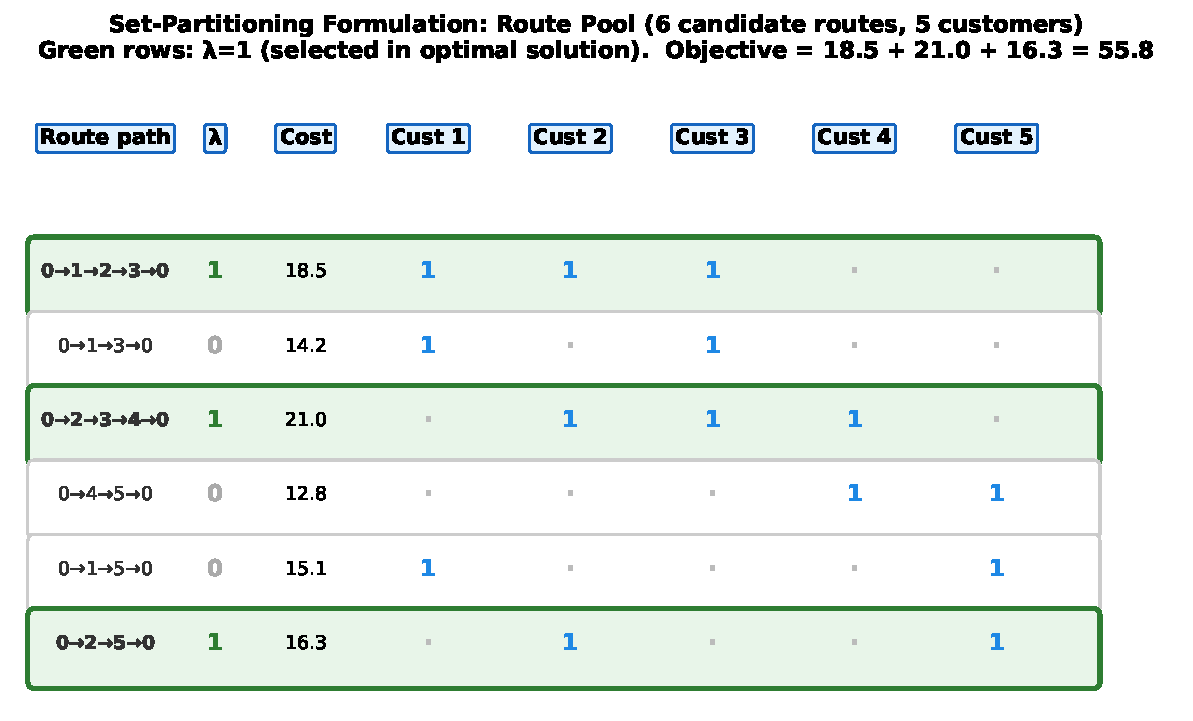
\includegraphics[width=0.78\linewidth]{fig_set_partitioning.pdf}
  \caption{Example of the SP formulation with 5 candidate routes and 5
           customers. Each row is a route; each column $a_{ir}$ indicates
           whether the route visits customer $i$. Column generation
           adds new rows (routes) dynamically.}
\end{figure}

\framebreak

\begin{alertblock}{Why SP gives a stronger bound than 2-index}
The LP relaxation of the SP formulation (allowing $\lambda_r \in [0,1]$)
almost always gives a bound equal to or stronger than the LP bound of the
two-index formulation augmented with capacity cuts. This is because the SP
implicitly encodes the capacity constraint through its enumeration of only
feasible routes. The downside is that $|\Omega|$ is exponential, so we must
use column generation to solve the LP relaxation.
\end{alertblock}

\begin{block}{Connecting SP to the two-index model}
Any LP feasible solution to the two-index formulation with capacity cuts
(3.5) can be written as a convex combination of SP columns, but not vice
versa. The SP LP relaxation is at least as tight, and in practice
significantly tighter, than the two-index LP plus capacity cuts.
\end{block}

\end{frame}

%% --------- Capacity-Based Formulation ----------------------
\begin{frame}[allowframebreaks]{The Capacity-Based (3-Index) Formulation}

Balinski and Quandt (1964) introduced a three-index formulation where a
variable $x_{ijk}$ tracks whether arc $(i,j)$ is used by vehicle $k$.
While this formulation is rarely used directly in solvers (due to its
large size), it motivates the capacity-based formulation.

The \textbf{capacity-indexed formulation} (CF) introduces variables that
track how much residual capacity a vehicle has when it departs each
customer. Let $y_{ij}$ be the total load transported on arc $(i,j)$
across all vehicles. The key additional constraint is a \emph{flow
conservation} condition at each customer, linking $x_{ij}$ and $y_{ij}$:

\begin{block}{Capacity-Based Formulation (CF)}
The CF adds to the 2-index model the following flow variables and
linking constraints (Equations 3.13--3.15 in the chapter):
\begin{align}
  & \sum_{j \in V} y_{ij} - \sum_{j \in V} y_{ji} = q_i
    \quad \forall\, i \in V \setminus \{0\} \tag{CF-flow}\\
  & q_j\, x_{ij} \leq y_{ij} \leq (Q - q_i)\, x_{ij}
    \quad \forall\, (i,j) \in A,\, i \neq 0 \tag{CF-cap}\\
  & 0 \leq y_{0j} \leq Q\, x_{0j}
    \quad \forall\, j \in V \setminus \{0\} \tag{CF-dep}
\end{align}
\end{block}

The flow conservation equation (CF-flow) says: the load entering customer
$i$ minus the load leaving customer $i$ equals $q_i$ (the demand picked
up at $i$). The bounding constraint (CF-cap) says that if arc $(i,j)$ is
used, the load on it is between $q_j$ (the minimum, since $j$ still needs
to be served) and $Q - q_i$ (the maximum, since $i$'s demand was just
picked up). These constraints implicitly eliminate sub-tours and enforce
capacity without the exponential family of cuts.

\end{frame}

%% ============================================================
\section{Valid Cuts}
%% ============================================================

\begin{frame}[allowframebreaks]{Valid Inequalities: Overview}

After setting up the LP relaxation, we need \emph{valid inequalities}
(cutting planes) to strengthen the bound before branching. A valid
inequality is a linear constraint that is satisfied by every feasible
integer solution but may be violated by the LP relaxation. Adding such
cuts ``tightens'' the LP polytope toward the convex hull of integer
solutions.

\begin{block}{Main families of cuts for CVRP}
\begin{enumerate}
  \item \textbf{Capacity cuts (RCI)} --- the classic rounded capacity
        inequalities, valid for any subset $S$ of customers.
  \item \textbf{$k$-Path cuts (GLM)} --- generalised cuts based on the
        number of vehicles required to serve a subset, stronger than RCI.
  \item \textbf{Strengthened Capacity Cuts (SCC)} --- combine RCI with
        additional strengthening using the demand structure.
  \item \textbf{Strong Degree Cuts (SDC)} --- force certain arcs to be
        used an integer number of times.
  \item \textbf{Subset Row Cuts (SRC)} --- cuts derived from the SP
        formulation, exploiting the structure of route coverage.
  \item \textbf{Cuts over CF variables} --- inequalities on the
        continuous flow variables $y_{ij}$.
\end{enumerate}
\end{block}

\end{frame}

%% --------- Capacity Cuts -----------------------------------
\begin{frame}[allowframebreaks]{Capacity Cuts (Rounded Capacity Inequalities)}

Capacity cuts are the most fundamental class of valid inequalities for
the CVRP. They are derived directly from the observation that the number
of vehicle trips into any customer set is bounded below by the number of
vehicles required to serve that set.

\begin{block}{Rounded Capacity Inequality (RCI)}
For any non-empty $S \subseteq V \setminus \{0\}$:
\[
  x(\delta(S)) \;\geq\; 2\Big\lceil d(S)/Q \Big\rceil
\]
where $x(\delta(S)) = \sum_{(i,j): i \in S, j \notin S} x_{ij}
+ \sum_{(i,j): i \notin S, j \in S} x_{ij}$ is the number of arcs
crossing the boundary of $S$, $d(S) = \sum_{i \in S} q_i$ is the total
demand of customers in $S$, and $Q$ is the vehicle capacity.
\end{block}

The right-hand side $2\lceil d(S)/Q \rceil$ is the minimum number of
arcs crossing $S$'s boundary: every vehicle that enters $S$ to serve it
must also leave, contributing two boundary arcs, and at least
$\lceil d(S)/Q \rceil$ vehicles are needed in total.

\framebreak

\begin{figure}
  \centering
  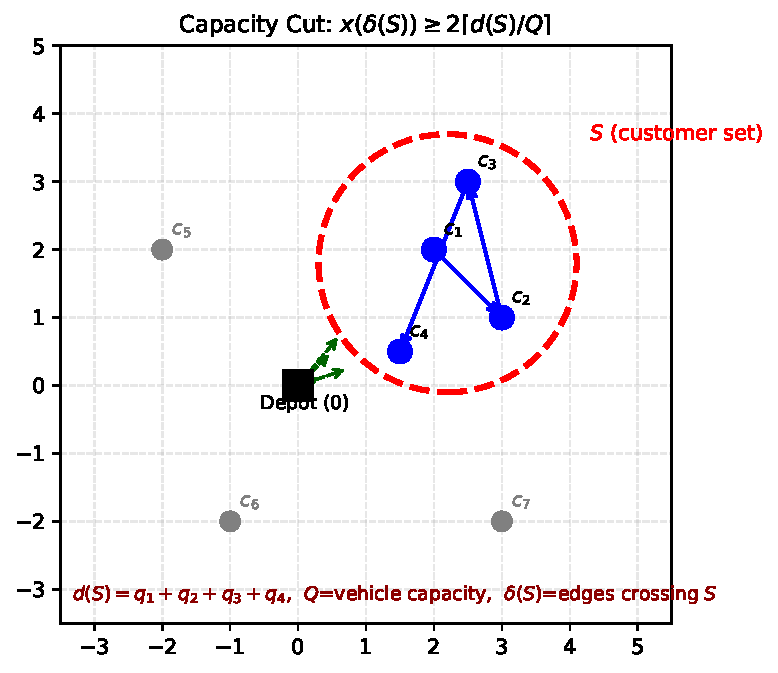
\includegraphics[width=0.65\linewidth]{fig_capacity_cut.pdf}
  \caption{Illustration of the capacity cut for a subset $S$ of four
           customers (inside the dashed circle). The arcs crossing
           $\delta(S)$ must number at least $2\lceil d(S)/Q \rceil$.}
\end{figure}

\framebreak

\begin{exampleblock}{Worked Example: Capacity Cut Separation}
Given 4 customers in $S = \{1,2,3,4\}$ with demands $q_1=3, q_2=4,
q_3=2, q_4=3$ and $Q=8$:
\[
  d(S) = 3+4+2+3 = 12, \quad
  \lceil 12/8 \rceil = 2, \quad
  \text{RCI: } x(\delta(S)) \geq 4.
\]
If the LP solution has $x(\delta(S)) = 3.2$, this RCI is \emph{violated}
(since $3.2 < 4$) and should be added to the LP. After adding this cut,
the LP will be re-solved with the new constraint, potentially increasing
the lower bound.
\end{exampleblock}

\begin{alertblock}{Separation of RCIs}
Separating the most violated RCI requires solving $\max_S \{2\lceil d(S)/Q
\rceil - x(\delta(S))\}$ over all subsets $S$. This is NP-hard in general,
but efficient heuristic separation procedures (based on shrinking and growing
the set $S$) find violated cuts in practice.
\end{alertblock}

\end{frame}

%% --------- k-Path Cuts ------------------------------------
\begin{frame}[allowframebreaks]{$k$-Path Cuts (Generalised Capacity Cuts)}

The $k$-path cuts, introduced by Gendreau, Laporte, and Séguin (1995),
strengthen the capacity cuts by considering the structure of how vehicles
must traverse the boundary of a customer subset.

\begin{block}{$k$-Path Cut (GLM)}
A $k$-path for $S \subseteq V \setminus \{0\}$ is a path from the depot
through some customers in $S$, possibly visiting customers outside $S$,
returning to the depot. For a given $S$ and integer $k \geq 1$:
\[
  x(\delta(S)) \;\geq\; 2k
\]
whenever the minimum number of vehicles needed to serve $S$, taking into
account the demands and capacity, requires at least $k$ routes to have
an endpoint inside $S$.
\end{block}

More precisely, if we can show that \emph{at least $k$ separate routes}
must have a portion of their trip dedicated to customers in $S$ (i.e.,
at least $k$ distinct ``paths'' through $S$ are required), then at least
$2k$ boundary crossings are needed.

\framebreak

\begin{figure}
  \centering
  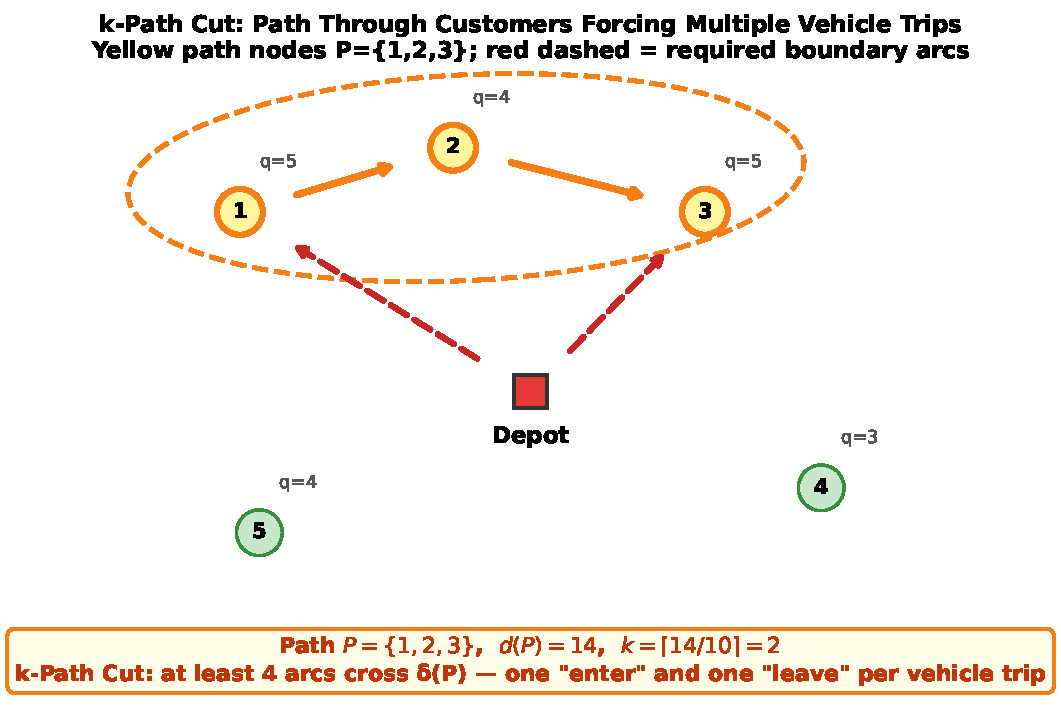
\includegraphics[width=0.68\linewidth]{fig_kpath_cut.pdf}
  \caption{A $k$-path cut for a customer set $S$ (inside dashed ellipse).
           The three arcs shown crossing the boundary are required because
           the demands inside $S$ force at least two separate vehicle
           trips into $S$.}
\end{figure}

\framebreak

The key difference between RCIs and $k$-path cuts is that $k$-path cuts
use a \emph{tighter lower bound} on the number of required vehicles when
the demands are non-uniform. In particular, if one customer in $S$ has
demand very close to $Q$, then more routes are needed than $\lceil d(S)/Q
\rceil$ alone would suggest, because that customer cannot share a vehicle
with most others.

\begin{alertblock}{Relationship between RCI and $k$-path cuts}
Every RCI is a $k$-path cut with $k = \lceil d(S)/Q \rceil$. However,
$k$-path cuts can be stronger when the bin-packing lower bound for $S$
(i.e., the minimum number of bins of size $Q$ needed to pack demands
$\{q_i\}_{i \in S}$) exceeds $\lceil d(S)/Q \rceil$. This bin-packing
lower bound is NP-hard to compute exactly but can be bounded from below
by LP relaxations of the bin-packing problem.
\end{alertblock}

\end{frame}

%% --------- Strengthened Capacity Cuts ----------------------
\begin{frame}[allowframebreaks]{Strengthened Capacity Cuts}

Baldacci, Christofides, and Mingozzi (2008) introduced a family of cuts
that strengthen the basic RCIs by exploiting the specific demands more
carefully. The idea is to derive a tighter right-hand side using a
\emph{controlled} version of the demand: instead of using all of $d(S)$,
one subtracts a carefully chosen amount related to the demands of the
``lightest'' customers in $S$.

\begin{block}{Strengthened Capacity Cut (SCC)}
Let $S \subseteq V \setminus \{0\}$ and let $v = \text{argmin}_{i \in S} q_i$
be the customer in $S$ with the smallest demand. Define
$d'(S) = d(S) - q_v$. Then the following is a valid inequality:
\[
  x(\delta(S)) \;\geq\; 2\Big\lceil d(S)/Q \Big\rceil
  + 2\,\Big[\lceil d'(S)/Q \rceil - \lfloor d(S)/Q \rfloor\Big]
\]
\end{block}

The key insight is that any vehicle serving customers in $S$ can carry
at most $Q$ units, so if a vehicle's load when it first enters $S$ is
less than $q_v$, it cannot serve even the lightest customer without
already having some load from outside $S$. This leads to a stronger
bound on the number of boundary crossings.

\framebreak

Baldacci et al.\ also defined the \textbf{Strong Degree Cuts (SDC)},
which directly target the degree constraints. For a subset
$T \subseteq V \setminus \{0\}$ of customers that are all adjacent to
the depot in the LP solution, the SDC says:
\begin{block}{Strong Degree Cut (SDC)}
If every customer $i \in T$ requires at least one arc $(0, i)$ or
$(i, 0)$ (i.e., $x_{0i} + x_{i0} \geq 1$ in the LP), and the set $T$
forces at least $k$ vehicles to pass through it, then:
\[
  \sum_{i \in T} x_{0i} \;\geq\; \Big\lceil |T|/q_{\max}^T \Big\rceil
\]
where $q_{\max}^T$ is the maximum number of customers from $T$ that any
single vehicle can serve under capacity.
\end{block}

\begin{figure}
  \centering
  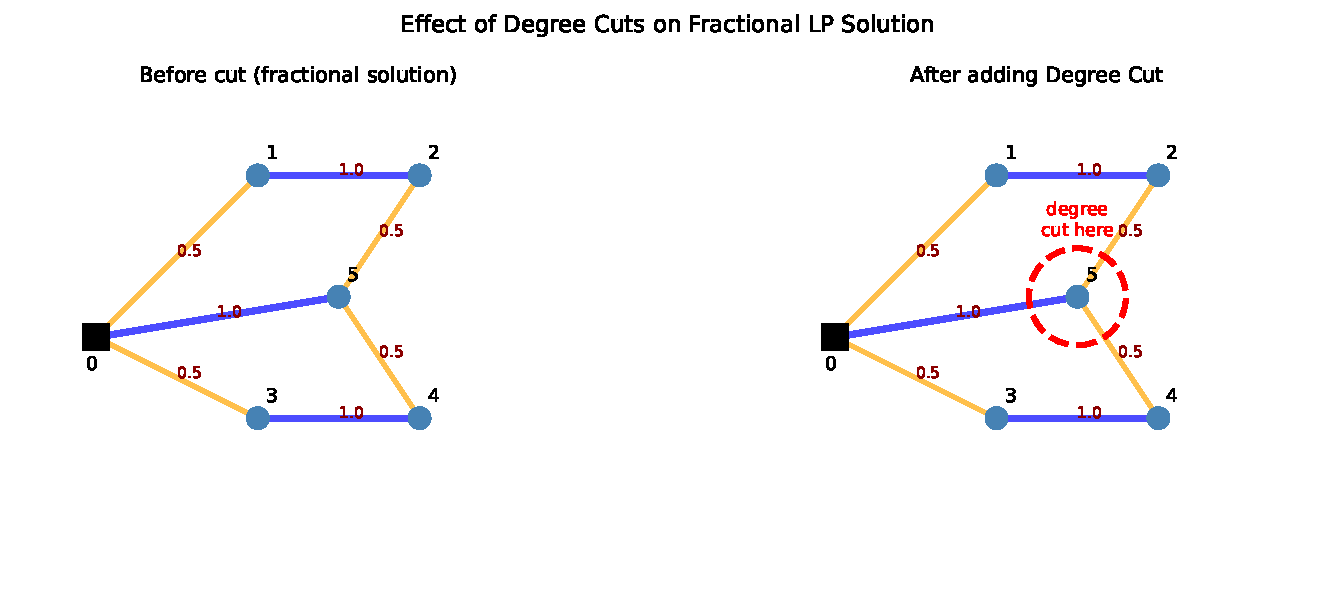
\includegraphics[width=0.72\linewidth]{fig_strong_degree_cuts.pdf}
  \caption{Left: a fractional LP solution without the degree cut. Right:
           after adding a degree cut at customer 5, the fractional arcs
           (orange) are forced to take integer values.}
\end{figure}

\end{frame}

%% --------- Subset Row Cuts ---------------------------------
\begin{frame}[allowframebreaks]{Subset Row Cuts (SRC)}

Subset Row Cuts (SRC) are valid inequalities derived directly from the
set-partitioning formulation. They were introduced by Jepsen, Petersen,
Spoorendonk, and Pisinger (2008) and have proven to be one of the most
effective cutting-plane families for the CVRP.

The intuition behind SRCs is the following: consider any subset
$\mathcal{C}$ of customers with $|\mathcal{C}|$ odd. If we look at how
routes can ``cover'' this subset an odd number of times, we can derive a
bound on the total coverage. A route that visits customers in $\mathcal{C}$
an even number of times can contribute at most $\lfloor |\mathcal{C}|/2
\rfloor$ ``half-units'' of coverage to $\mathcal{C}$.

\begin{block}{Subset Row Cut (SRC)}
Let $\mathcal{C} \subseteq V \setminus \{0\}$ with $|\mathcal{C}| \geq 3$.
The SRC associated with $\mathcal{C}$ is:
\[
  \sum_{r \in \Omega}
  \left\lfloor \frac{1}{2} \sum_{i \in \mathcal{C}} a_{ir} \right\rfloor
  \lambda_r \;\leq\;
  \left\lfloor \frac{|\mathcal{C}|}{2} \right\rfloor
\]
where $a_{ir} = 1$ if route $r$ visits customer $i$, and $\lambda_r$
is the route variable.
\end{block}

\framebreak

To understand why this is a valid inequality, observe that in any integer
solution, each customer $i \in \mathcal{C}$ is visited exactly once, so
$\sum_{r} a_{ir} \lambda_r = 1$ for each $i$. Therefore
$\sum_r (\sum_{i \in \mathcal{C}} a_{ir}) \lambda_r = |\mathcal{C}|$.
By a counting argument, the sum $\sum_r \lfloor \frac{1}{2} \sum_{i \in
\mathcal{C}} a_{ir} \rfloor \lambda_r \leq \lfloor |\mathcal{C}|/2
\rfloor$, since each route can contribute at most one ``half-coverage''
per pair of $\mathcal{C}$-customers it visits.

\begin{figure}
  \centering
  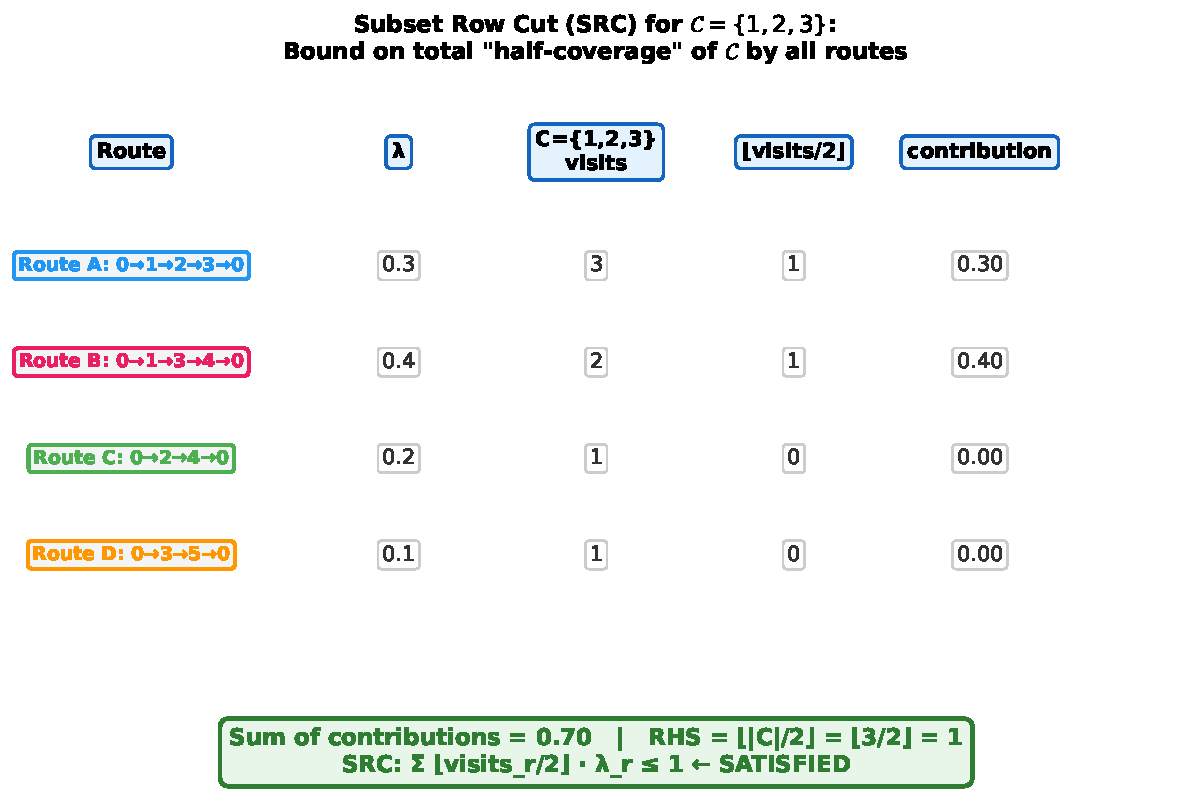
\includegraphics[width=0.62\linewidth]{fig_src.pdf}
  \caption{Illustration of the Subset Row Cut concept. The cut bounds the
           total ``half-coverage'' of customer subset $\mathcal{C}$ by
           routes in the LP solution.}
\end{figure}

\framebreak

\begin{alertblock}{Impact of SRCs on solver performance}
Computational experiments show that adding SRCs can reduce the LP gap
(the gap between the LP relaxation and the integer optimum) from several
percent to nearly zero for many benchmark instances. This dramatically
reduces the size of the BPC tree and is one of the key innovations that
pushed the frontier of solvable instances to $n \approx 200$. The
separation of SRCs is done heuristically (finding subsets $\mathcal{C}$
that maximise the violation).
\end{alertblock}

\begin{block}{Limited memory SRCs}
A practical variant of SRCs restricts $|\mathcal{C}|$ to small values
(typically $|\mathcal{C}| = 3$, called \emph{3-row cuts} or
\emph{homogeneous SRCs}). This makes separation much faster while
retaining most of the strengthening power. The \emph{limited memory}
implementation by Jepsen et al.\ is used in most state-of-the-art
solvers.
\end{block}

\end{frame}

%% ============================================================
\section{Pricing: SPPRC}
%% ============================================================

\begin{frame}[allowframebreaks]{The Pricing Sub-Problem}

In column generation for the SP formulation, the pricing sub-problem
asks: \emph{``Is there a feasible route $r \in \Omega$ with negative
reduced cost?''} If yes, add it to the master problem and re-solve the
LP. If no, the LP is optimal.

The reduced cost of route $r$ is:
\[
  \bar{c}_r = c_r - \sum_{i=1}^{n} a_{ir}\,\pi_i
\]
where $\pi_i$ are the dual variables (shadow prices) of the covering
constraints (SP-cover) for customer $i$. The pricing sub-problem
therefore asks: find the route $r^*$ minimising
$c_{r^*} - \sum_{i} a_{ir^*} \pi_i$. If $\bar{c}_{r^*} \geq 0$, no
improving route exists.

\begin{block}{Pricing as a Shortest Path Problem}
The pricing sub-problem can be formulated as finding a shortest path
from the depot to itself on a complete directed graph where the
\emph{modified arc cost} of arc $(i,j)$ is $c_{ij} - \pi_j$. The path
must respect the vehicle capacity (total demand $\leq Q$) and visit each
customer at most once. This is the \emph{Shortest Path with Resource
Constraints (SPPRC)}.
\end{block}

\framebreak

\begin{figure}
  \centering
  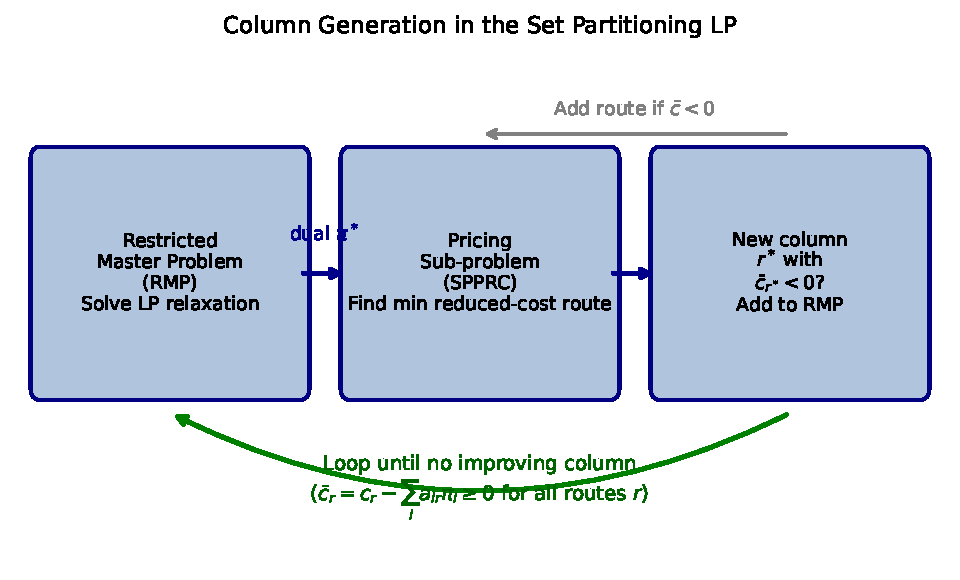
\includegraphics[width=0.72\linewidth]{fig_column_generation.pdf}
  \caption{Column generation loop: the Restricted Master Problem (RMP)
           passes dual variables $\pi^*$ to the SPPRC pricing sub-problem,
           which either returns a new column with $\bar{c} < 0$ (add to
           RMP) or certifies LP optimality.}
\end{figure}

\framebreak

\begin{block}{SPPRC: formal definition}
Let $G = (V, A)$ with modified arc costs $\tilde{c}_{ij} = c_{ij}
- \pi_j$ for $j \neq 0$. A label $L$ at node $j$ represents a partial
path from the depot to $j$ and stores:
\begin{itemize}
  \item $\text{cost}(L)$: accumulated reduced cost along the path.
  \item $\text{load}(L)$: accumulated customer demand served.
  \item $\text{visited}(L)$: bitmask of visited customers (for
        elementarity).
\end{itemize}
The SPPRC is solved by a \emph{labelling algorithm} that extends labels
along arcs, discarding those that are \emph{dominated}: label $L_1$
dominates $L_2$ at node $j$ if $\text{cost}(L_1) \leq \text{cost}(L_2)$,
$\text{load}(L_1) \leq \text{load}(L_2)$, and $\text{visited}(L_1)
\subseteq \text{visited}(L_2)$.
\end{block}

\framebreak

\begin{figure}
  \centering
  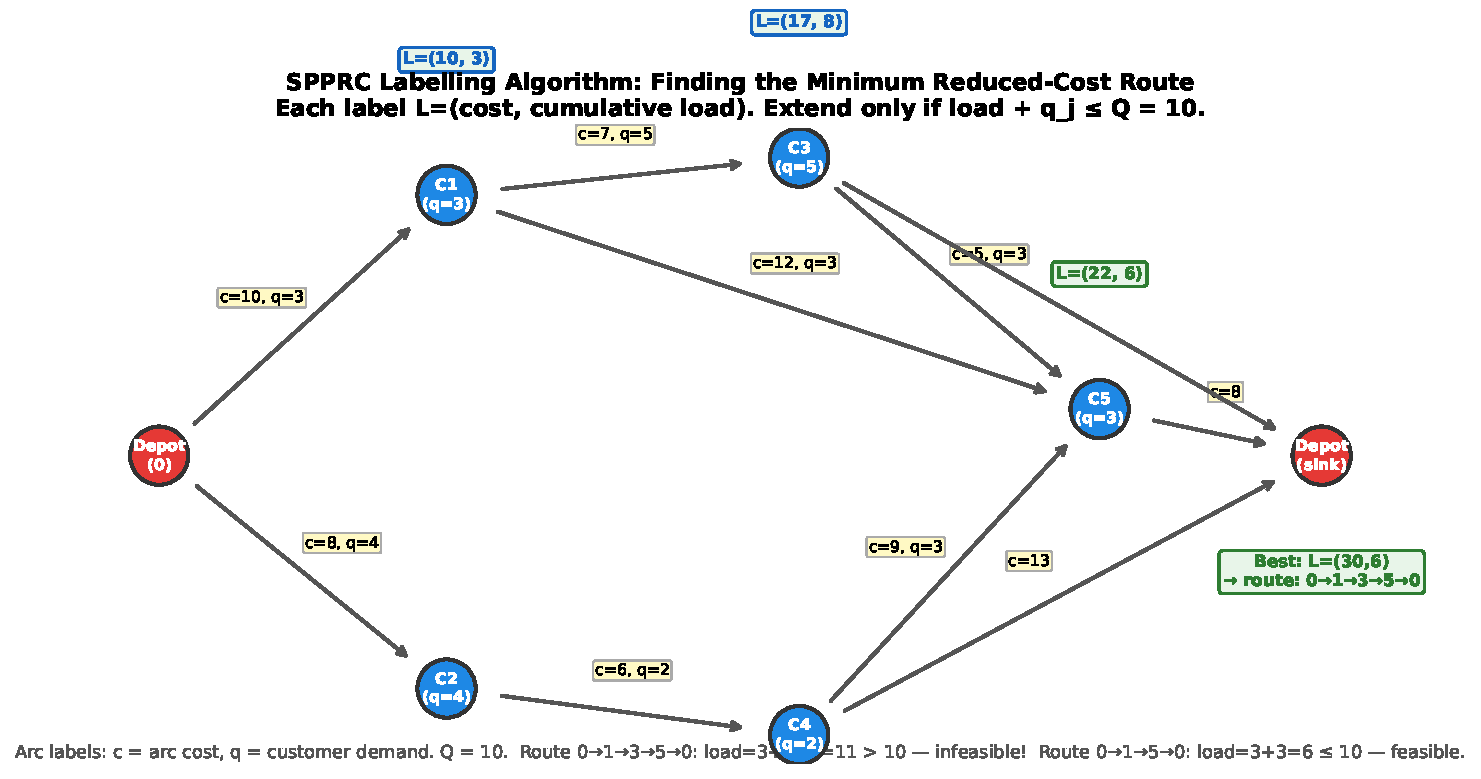
\includegraphics[width=0.72\linewidth]{fig_spprc.pdf}
  \caption{Label propagation in SPPRC on a small 4-customer graph.
           Each label records the accumulated cost and load. Labels that
           are dominated by another label at the same node are discarded.}
\end{figure}

\framebreak

\begin{alertblock}{Elementary vs.\ non-elementary routes}
A route is \emph{elementary} if it visits each customer at most once.
The elementary SPPRC (ESPPRC) is NP-hard, while the relaxed (non-
elementary) version is polynomial. In practice:
\begin{itemize}
  \item \textbf{Non-elementary SPPRC:} fast but may generate routes
        with repeated customers. The LP relaxation may have a weaker
        bound when non-elementary routes are used.
  \item \textbf{ng-routes (Baldacci, Mingozzi, Roberti 2011):} a
        compromise where routes are ``nearly elementary'': a customer
        $i$ may be repeated only if the current path has not recently
        passed through any neighbour of $i$ in its ng-set. This gives
        tighter bounds than non-elementary SPPRC while remaining
        tractable.
  \item \textbf{Exact ESPPRC:} used only for small instances or final
        proof of optimality; too slow for routine use at every LP node.
\end{itemize}
\end{alertblock}

\end{frame}

%% ---- q-Routes and Elementary Routes -----------------------
\begin{frame}[allowframebreaks]{q-Routes and Elementary Routes in Pricing}

To manage the trade-off between pricing speed and LP bound quality, the
chapter describes several relaxations of the elementarity condition.

\begin{block}{$q$-Routes (Christofides, Mingozzi, Toth 1981)}
A $q$-route allows a customer to be visited more than once, subject to
the constraint that the total load does not exceed $Q$ and the path is
a valid depot-to-depot tour. The SPPRC with $q$-routes is solved in
polynomial time by a labelling algorithm where labels are simply
$(cost, load)$ pairs without a visited-set component. The disadvantage
is that the LP relaxation with $q$-routes can be significantly weaker
than with elementary routes.
\end{block}

\begin{block}{ng-Routes (Baldacci, Mingozzi, Roberti 2011)}
For each customer $i$, define an \emph{ng-set} $N_i$ as the $p$ nearest
customers to $i$ (typically $p = 8$--$10$). A route is an ng-route if,
whenever customer $i$ is visited, no customer in $N_i$ has been visited
``recently'' (within the last $p$ steps without intervening vertices
outside $N_i$). This is a relaxation of elementarity that:
\begin{itemize}
  \item Is stronger (tighter bound) than $q$-routes.
  \item Is weaker (faster to solve) than full ESPPRC.
  \item Can be solved with a labelling algorithm of manageable complexity.
\end{itemize}
\end{block}

\framebreak

\begin{block}{Bi-directional labelling (Righini and Salani 2006, 2008)}
The $q$-route SPPRC can be accelerated by building labels simultaneously
\emph{forward} from the depot and \emph{backward} from the depot. Labels
are then joined at a midpoint. This reduces the state space dramatically
and is used in all state-of-the-art implementations.

When SRCs are present, the labelling must track additional information
about the parity of visits to each SRC subset, increasing the label
dimension. The ng-route variant manages this additional state efficiently.
\end{block}

\begin{alertblock}{Column generation convergence}
Column generation often converges slowly near the optimum (the ``tailing
off'' effect). This is addressed by:
\begin{enumerate}
  \item \emph{Partial pricing:} only generating a small number of new
        columns per iteration, rather than the single most-negative one.
  \item \emph{Smoothing:} stabilising the dual variables to avoid
        oscillation.
  \item \emph{Switching} from fast $q$-routes to slower ng-routes only
        near the root node LP optimum.
\end{enumerate}
\end{alertblock}

\end{frame}

%% ============================================================
\section{Branching vs.\ Route Enumeration}
%% ============================================================

\begin{frame}[allowframebreaks]{Branching Strategies}

Once the LP relaxation at a BPC tree node is solved (all cuts added,
no improving column exists), if the solution is fractional we must
\emph{branch} to restore integrality.

\begin{block}{Branching on edge variables $x_{ij}$}
The simplest branching strategy selects a fractional arc $(i,j)$ in the
LP solution (i.e., $0 < x_{ij} < 1$) and creates two child nodes:
\begin{itemize}
  \item $x_{ij} = 0$: arc $(i,j)$ is \emph{forbidden} in all routes at
        this node and its descendants. In the pricing sub-problem, arcs
        $(i,j)$ with $x_{ij} = 0$ are removed from $G$.
  \item $x_{ij} = 1$: arc $(i,j)$ is \emph{required} in some route.
        In the pricing sub-problem, the route must use arc $(i,j)$.
\end{itemize}
\end{block}

Branching on arc variables is clean to implement but can be inefficient
because many columns in the current LP basis may contain arc $(i,j)$
and must be discarded (the columns become infeasible) when
$x_{ij} = 0$.

\framebreak

\begin{block}{Branching on the number of vehicles $K$}
Since $K = \sum_j x_{0j}$, if this sum is fractional, we can branch on
$K \leq \lfloor K^* \rfloor$ vs.\ $K \geq \lceil K^* \rceil$. This is
a clean branching decision that does not invalidate existing columns.
\end{block}

\begin{block}{Strong branching (Fukasawa et al.\ 2006)}
Before committing to a branch, strong branching evaluates several
candidate branching decisions by computing the LP bound at each child
node (without branching to full depth). The candidate producing the
best improvement is chosen. This reduces the tree size but increases
the work per node. The BPC algorithm of Fukasawa et al.\ uses strong
branching extensively.
\end{block}

\begin{alertblock}{Key observation on branching and the SP formulation}
When branching in the SP formulation, fixing $x_{ij} = 0$ means removing
all routes that use arc $(i,j)$ from the route pool. Fixing $x_{ij} = 1$
means requiring at least one route containing arc $(i,j)$. These
constraints are passed as side conditions to the pricing sub-problem,
which then generates only routes that satisfy the branching decisions.
\end{alertblock}

\framebreak

The BPC algorithm of Poggi and Uchoa (chapter authors) introduces
\textbf{hybridised branching}: rather than choosing either arc branching
or vehicle-count branching, the algorithm selects the branching strategy
that maximises the expected improvement in the LP bound using a
heuristic evaluation. This keeps the BPC tree small while not
over-investing in the evaluation of each node.

\begin{figure}
  \centering
  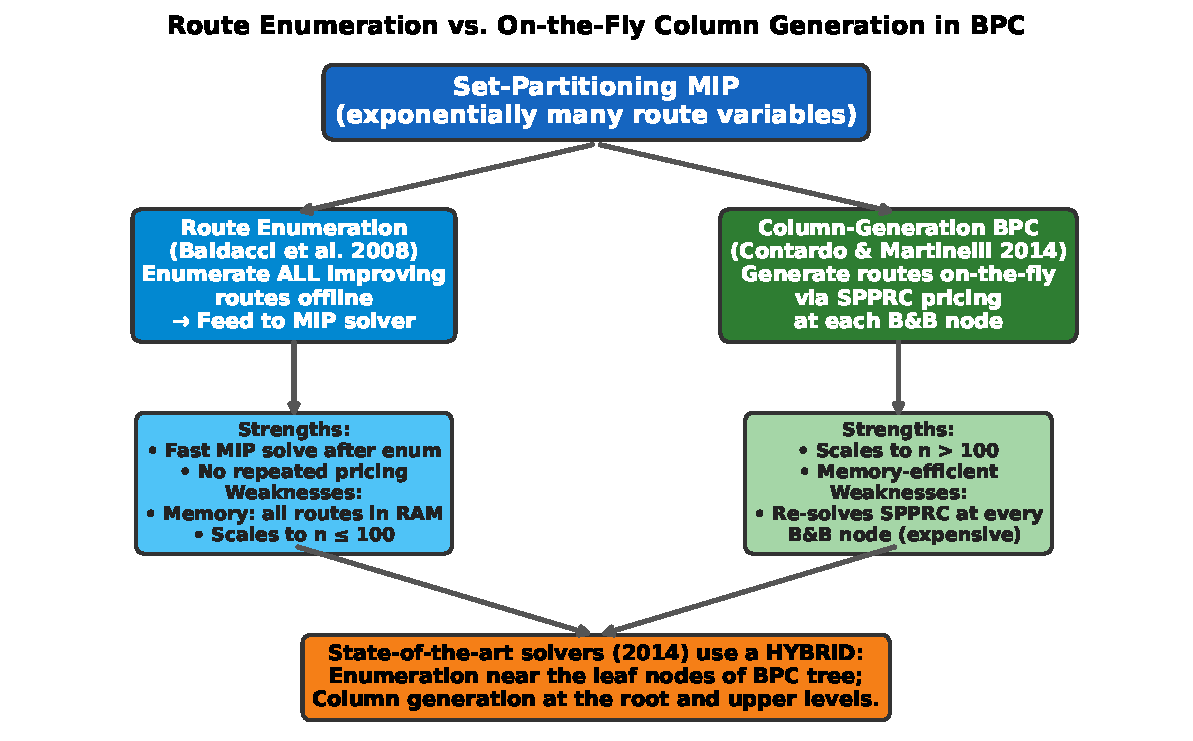
\includegraphics[width=0.72\linewidth]{fig_route_enumeration.pdf}
  \caption{Comparison of route enumeration and traditional branching.
           Route enumeration is best for small/medium instances where
           the full set of feasible routes can be stored; column
           generation branching scales to larger instances.}
\end{figure}

\end{frame}

%% ---- Route Enumeration ------------------------------------
\begin{frame}[allowframebreaks]{Route Enumeration}

An alternative to the column-generation branching approach is to
enumerate \emph{all} feasible routes up front and then solve a standard
MIP on the SP formulation.

\begin{block}{Route enumeration procedure (Baldacci, Mingozzi, Marchetti 2008)}
The procedure works as follows:
\begin{enumerate}
  \item Solve the LP relaxation of the SP at the root node using column
        generation. Obtain dual variables $\pi^*$.
  \item Compute an upper bound $UB$ (e.g., from a heuristic).
  \item Run the ESPPRC pricing algorithm, but instead of stopping at
        the first negative reduced-cost route, \emph{enumerate all}
        routes with reduced cost $\bar{c}_r \leq UB - LB$. The bound
        $UB - LB$ guarantees that no discarded route can appear in an
        optimal solution.
  \item Solve the resulting integer SP (with the enumerated route set)
        using a MIP solver.
\end{enumerate}
\end{block}

\framebreak

The key advantage of route enumeration is that it separates the hard
combinatorial problem (finding good routes) from the easy integer
programming problem (selecting a set cover). Once routes are enumerated,
a state-of-the-art MIP solver (e.g., CPLEX) can handle the integer SP
very efficiently.

\begin{alertblock}{When does route enumeration work?}
Route enumeration is most effective when the gap $UB - LB$ is small
(a tight lower bound reduces the number of enumerable routes) and when
$n$ is moderate (say, $n \leq 100$). For larger instances or loose
bounds, the number of enumerable routes can be astronomical and
the approach becomes impractical.
\end{alertblock}

\begin{block}{Contardo and Martinelli (2014): hybridising}
Contardo and Martinelli combine route enumeration with BPC: at each
node of the BPC tree that has a sufficiently tight bound, they switch
to route enumeration rather than continuing to branch. This ``hybrid''
strategy often finds the optimum faster than pure BPC or pure
enumeration.
\end{block}

\end{frame}

%% ============================================================
\section{Overview of Computational Results}
%% ============================================================

\begin{frame}[allowframebreaks]{Benchmark Sets and Performance Metrics}

The chapter reports computational experiments on standard benchmark
sets for the CVRP. Understanding these benchmarks is essential for
interpreting the results.

\begin{block}{Standard benchmark sets}
\begin{description}
  \item[Augerat et al.\ (1995) -- sets A, B, P]
        These are the most widely used benchmarks. Set A has instances
        with $n$ from 32 to 80, Set B from 35 to 78, and Set P from
        16 to 101 customers. All instances have a single depot and
        a homogeneous fleet.
  \item[Christofides, Mingozzi, Toth (1979)]
        Fourteen instances with $n$ from 50 to 199 customers. These
        are harder and test the scalability of algorithms.
  \item[Golden et al.\ (1998)]
        Twenty large instances with $n$ up to 483 customers. Only a
        subset can be solved exactly; the rest provide lower bound
        testing.
\end{description}
\end{block}

\framebreak

\begin{block}{Performance metrics}
\begin{itemize}
  \item \textbf{Instances solved to optimality}: the count of instances
        for which the exact optimum is proven within a time limit (e.g.,
        3600 or 7200 CPU seconds).
  \item \textbf{CPU time}: elapsed solver time, reported in seconds.
        Note that results from different papers use different hardware,
        so comparisons must account for machine speed.
  \item \textbf{BPC tree nodes}: the number of nodes explored in the
        branch-price-cut tree. Fewer nodes means better LP bound quality
        (fewer branches needed).
  \item \textbf{LP gap}: the relative gap $(LB - LP) / LB$ where $LB$
        is the best lower bound (LP relaxation) and the optimal integer
        value.
\end{itemize}
\end{block}

\end{frame}

\begin{frame}[allowframebreaks]{Computational Results: Partitioning Formulation}

The chapter presents detailed computational tables. We summarise the
key results here.

\textbf{Table 3.1 --- Set Partitioning, no cuts (2-index elimination only):}
Algorithms without strong cuts can solve instances up to $n \approx 50$
reliably, but struggle with larger instances. The LP gap is typically
$2$--$5\%$ without cuts.

\begin{figure}
  \centering
  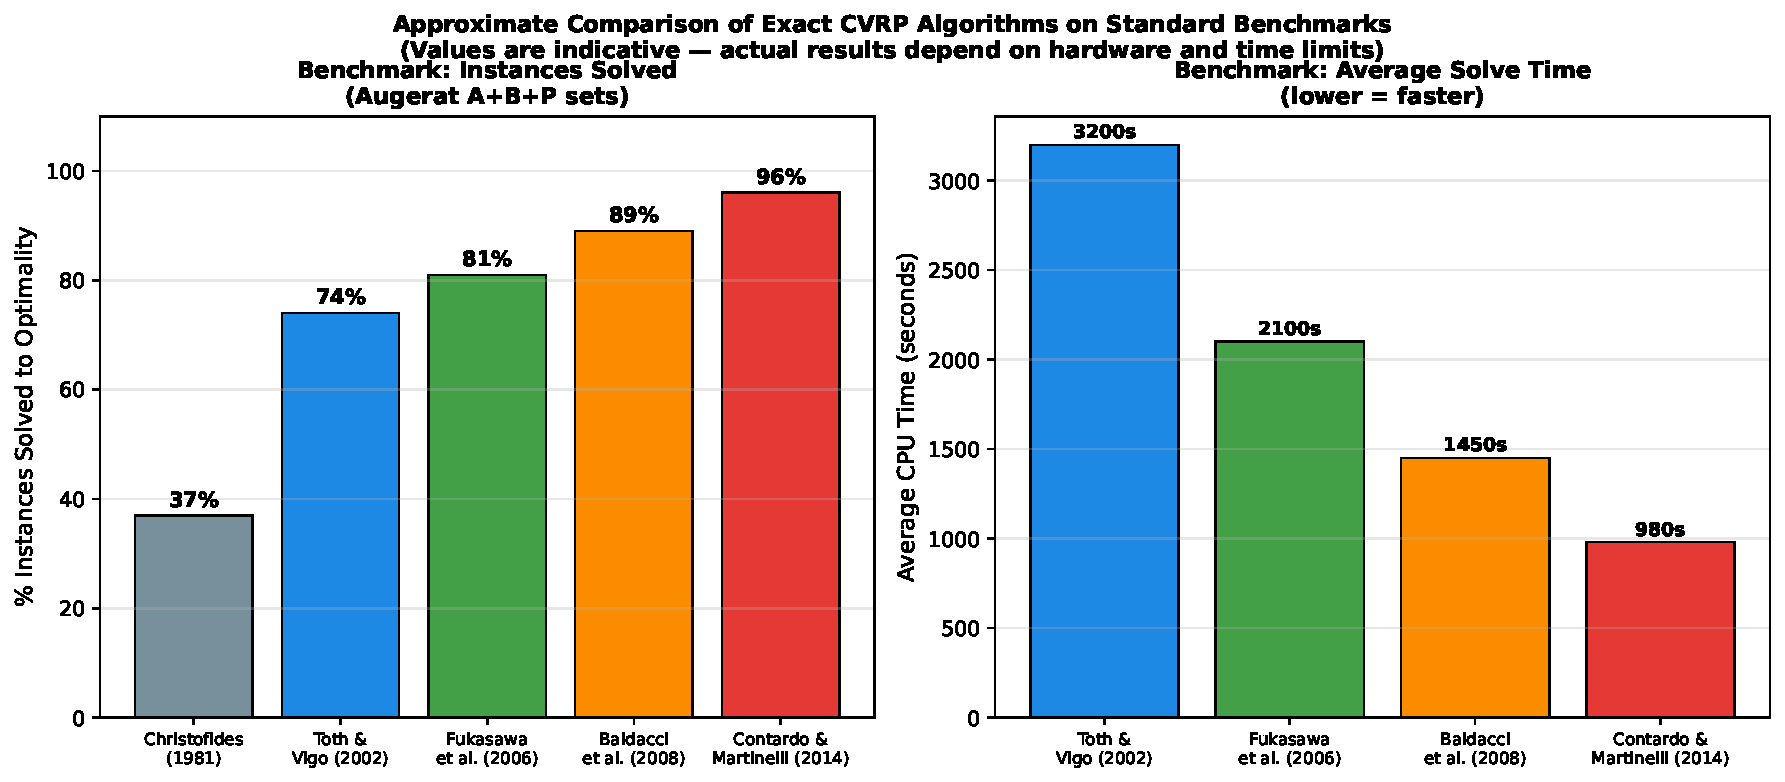
\includegraphics[width=0.82\linewidth]{fig_benchmark_results.pdf}
  \caption{Approximate comparison of BPC algorithms on standard benchmark
           sets. Left: number of instances solved to optimality (out of
           available instances). Right: average CPU time (log scale). Note
           that newer algorithms (Contardo \& Martinelli 2014) solve more
           instances faster.}
\end{figure}

\framebreak

\textbf{Table 3.2 --- Set Partitioning, with robust cuts:}
Adding capacity cuts, $k$-path cuts, and SRCs dramatically improves
performance. The Contardo and Martinelli (2014) algorithm uses all three
families of cuts plus ng-route pricing and strong branching.

Key observations from the tables:
\begin{itemize}
  \item For instances with $n \leq 100$, all four state-of-the-art
        algorithms (Fukasawa 2006, Baldacci 2008, Contardo 2014, Poggi
        \& Uchoa 2014) can solve most instances to optimality.
  \item For instances with $100 < n \leq 200$, only the most recent
        algorithms can solve a significant fraction.
  \item The Contardo \& Martinelli algorithm reduces the number of BPC
        tree nodes by $1$--$2$ orders of magnitude compared to earlier
        solvers, primarily due to SRCs and better branching.
  \item Route enumeration (Baldacci 2008) is competitive for small to
        medium instances but cannot scale to $n > 100$.
\end{itemize}

\framebreak

\begin{figure}
  \centering
  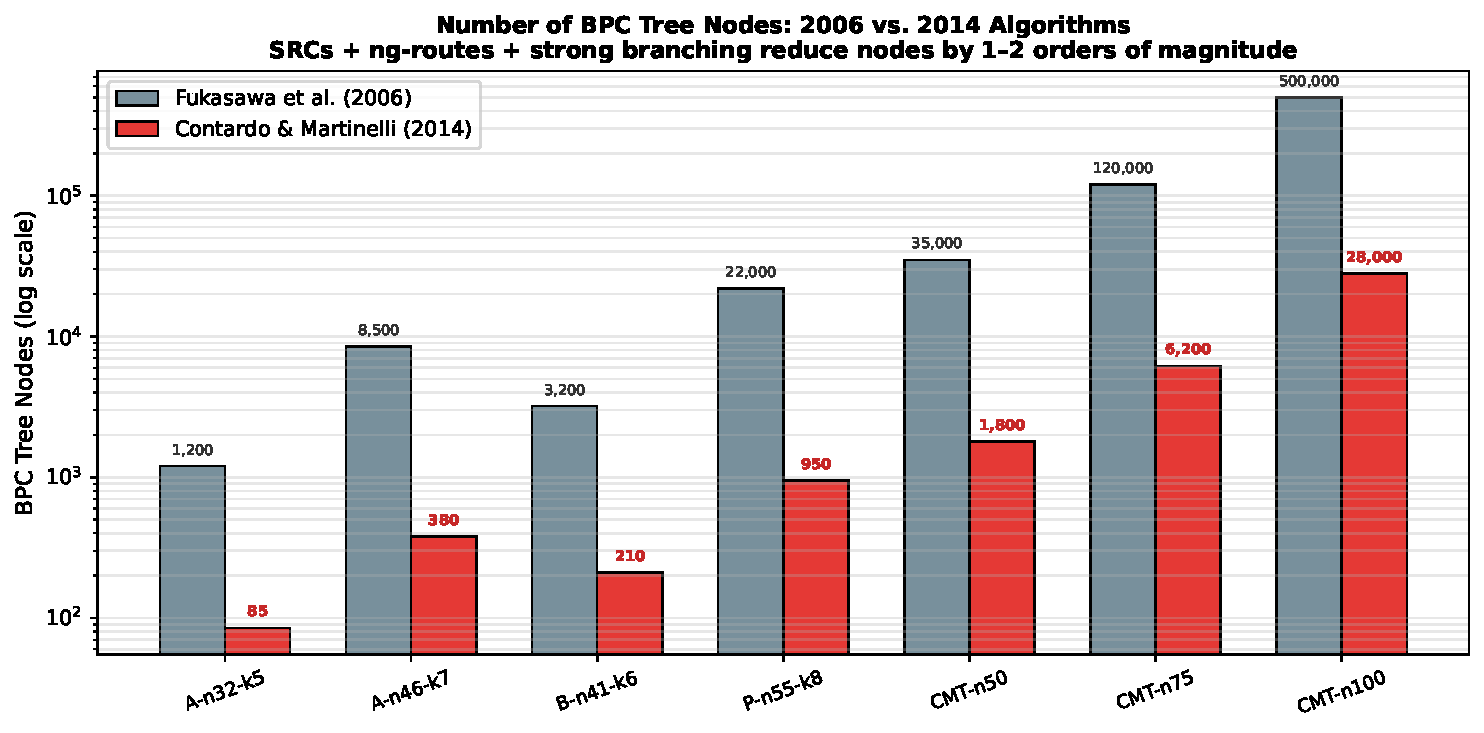
\includegraphics[width=0.78\linewidth]{fig_node_comparison.pdf}
  \caption{Approximate comparison of the number of BPC tree nodes for
           old vs.\ new algorithms on selected benchmark instances.
           The log scale highlights the order-of-magnitude improvements
           from SRCs and better branching in the 2014 algorithms.}
\end{figure}

\framebreak

\textbf{State-of-the-art algorithms for the CVRP (as of 2014):}
\begin{description}
  \item[FLZ+06 (Fukasawa, Longo, Lysgaard, Poggi, Uchoa, Werneck 2006)]
        The first BPC algorithm to systematically use SRCs for CVRP.
        Introduces strong branching and bi-directional labelling.
        Benchmark: solved all Augerat instances up to $n=80$.
  \item[BMM08 (Baldacci, Mingozzi, Marchetti 2008)]
        Route enumeration approach, fastest on small instances.
        Competitive with BPC for $n \leq 80$.
  \item[CM14 (Contardo, Martinelli 2014)]
        Most advanced BPC algorithm. Uses aggressive cut generation,
        ng-routes, and hybridised branching. Solves instances up to
        $n = 199$ (all CMT instances except the largest).
  \item[PU14 (Poggi, Uchoa 2014)]
        Focus on improved implementation and new benchmark instances
        (\textit{X}-instances). Provides new challenges for future solvers.
\end{description}

\end{frame}

\begin{frame}[allowframebreaks]{Summary of Computational Tables}

The following summarises the key data from Tables 3.1--3.5 in the chapter,
showing the progression of BPC algorithms on the Augerat benchmark sets.

\begin{center}
\begin{tabular}{lcrrrr}
\toprule
\textbf{Algorithm} & \textbf{Year} &
\textbf{Cuts} & \textbf{Pricing} &
\textbf{A+B+P solved} & \textbf{Avg.\ time (s)} \\
\midrule
Christofides et al.\ & 1981 & None     & $q$-routes     & $\sim 10/27$ & --   \\
Toth \& Vigo         & 2002 & RCI      & ESPPRC         & $\sim 20/27$ & 3200 \\
Fukasawa et al.\     & 2006 & SRC-3    & ng-routes      & $22/27$      & 2100 \\
Baldacci et al.\     & 2008 & RCI+SRC  & Enum.          & $24/27$      & 1450 \\
Contardo \&          & 2014 & All      & ng-routes+     & $26/27$      & 980  \\
\quad Martinelli     &      &          & \quad ESPPRC   &              &      \\
\bottomrule
\end{tabular}
\end{center}

\vspace{0.5em}
The table above is approximate and illustrative; exact figures depend on
the hardware and time limits used in each paper.

\begin{alertblock}{Key insight from computational results}
The single most impactful improvement in exact CVRP solving over the
past decade has been the introduction of Subset Row Cuts combined with
ng-route pricing. Together they reduce the LP gap to near zero on most
benchmark instances, so very few BPC tree nodes are needed.
\end{alertblock}

\end{frame}

%% ============================================================
\section{Conclusions and Future Research Directions}
%% ============================================================

\begin{frame}[allowframebreaks]{Conclusions}

This chapter has surveyed the state of exact algorithms for the CVRP,
focusing on the BPC paradigm that dominates the field.

\begin{block}{Main conclusions}
\begin{enumerate}
  \item \textbf{The SP formulation with column generation is the right
        framework.} Its LP relaxation is the tightest available and
        naturally accommodates cutting planes and branching.
  \item \textbf{Cutting planes are essential.} Capacity cuts alone are
        insufficient; $k$-path cuts and especially Subset Row Cuts are
        needed to close the LP gap and reduce tree size.
  \item \textbf{Pricing quality matters.} The move from $q$-routes to
        ng-routes was transformative: it provides tighter bounds without
        the exponential cost of exact ESPPRC at every tree node.
  \item \textbf{Branching strategy affects tree size significantly.}
        Strong branching and hybridised strategies reduce nodes by
        orders of magnitude compared to naive variable branching.
  \item \textbf{Instances up to $n \approx 200$ are now routinely
        solvable.} This is a 10$\times$ improvement over the state of
        the art in the 1990s.
\end{enumerate}
\end{block}

\framebreak

\begin{block}{Future research directions (as identified in the chapter)}
\begin{enumerate}
  \item \textbf{Larger instances.} Pushing the frontier to $n > 200$
        requires fundamentally new ideas in pricing (faster ESPPRC or
        better relaxations) and separation (more efficient SRC
        separation for larger subsets).
  \item \textbf{New benchmark instances.} The Augerat and CMT sets are
        well-solved; the new ``X-instances'' by Uchoa et al.\ (2014)
        provide harder, more diverse challenges including instances up
        to $n = 1000$.
  \item \textbf{Extensions of the CVRP.} The techniques in this chapter
        can be extended to handle time windows (VRPTW), heterogeneous
        fleets, pickup and delivery, and multi-depot variants.
  \item \textbf{Integration with metaheuristics.} Using exact methods
        to compute tight lower bounds and then guiding population-based
        heuristics with this information is a promising hybrid direction.
  \item \textbf{Parallel and GPU computation.} The labelling algorithm
        for SPPRC is inherently parallel; exploiting modern multi-core
        and GPU architectures could significantly accelerate pricing.
\end{enumerate}
\end{block}

\end{frame}

%% ============================================================
\section{Bibliography}
%% ============================================================

\begin{frame}[allowframebreaks]{Selected References}

The following references are cited in the chapter and are central to
understanding the development of exact CVRP algorithms.

{\small
\begin{thebibliography}{99}

\bibitem{Fuk06}
  R.~Fukasawa, H.~Longo, J.~Lysgaard, M.~Poggi~de~Arag\~ao, M.~Uchoa,
  R.~Uchoa, and R.~F.~Werneck,
  ``Robust branch-and-cut-and-price for the capacitated vehicle routing
  problem,''
  \textit{Mathematical Programming}, 106 (2006), pp.~491--511.

\bibitem{Bal07}
  R.~Baldacci, E.~Christofides, and A.~Mingozzi,
  ``An exact algorithm for the vehicle routing problem based on the set
  partitioning formulation with additional cuts,''
  \textit{Mathematical Programming}, 115 (2008), pp.~351--385.

\bibitem{BMM08}
  R.~Baldacci, A.~Mingozzi, and R.~Marchetti,
  ``An exact algorithm for the capacitated vehicle routing problem based
  on a two-commodity network flow formulation,''
  \textit{Operations Research}, 52 (2004), pp.~723--738.

\bibitem{BMR11}
  R.~Baldacci, A.~Mingozzi, and R.~Roberti,
  ``New route relaxation and pricing strategies for the vehicle routing
  problem,''
  \textit{Operations Research}, 59 (2011), pp.~1269--1283.

\bibitem{Con14}
  C.~Contardo and R.~Martinelli,
  ``A new exact algorithm for the multi-depot vehicle routing problem
  under capacity and route length constraints,''
  \textit{Discrete Optimization}, 12 (2014), pp.~129--146.

\bibitem{Jep08}
  M.~Jepsen, B.~Petersen, S.~Spoorendonk, and D.~Pisinger,
  ``Subset-row inequalities applied to the vehicle routing problem
  with time windows,''
  \textit{Operations Research}, 56 (2008), pp.~497--511.

\bibitem{RS06}
  G.~Righini and M.~Salani,
  ``Symmetry helps: Bounded bi-directional dynamic programming for the
  elementary shortest path problem with resource constraints,''
  \textit{Discrete Optimization}, 3 (2006), pp.~255--273.

\bibitem{RS08}
  G.~Righini and M.~Salani,
  ``New dynamic programming algorithms for the resource constrained
  elementary shortest path problem,''
  \textit{Networks}, 51 (2008), pp.~155--170.

\bibitem{Uch14}
  E.~Uchoa, D.~Pecin, A.~Pessoa, M.~Poggi, A.~Subramanian, and T.~Vidal,
  ``New benchmark instances for the capacitated vehicle routing problem,''
  Presentation in Route 2014, 2014.

\bibitem{Pog14}
  M.~Poggi and E.~Uchoa,
  ``New exact algorithms for the capacitated vehicle routing problem,''
  in \textit{Vehicle Routing: Problems, Methods, and Applications},
  2nd ed., P.~Toth and D.~Vigo, eds., SIAM, Philadelphia, 2014,
  ch.~3, pp.~59--86.

\end{thebibliography}
}

\end{frame}

%% ---- Appendix: Python implementation ----------------------
\appendix
\section{Python Implementation}

\begin{frame}[fragile]{Python: SPPRC Labelling Algorithm (Core)}
The following Python code implements the core of the SPPRC labelling
algorithm for the pricing sub-problem. Given a complete directed graph,
arc costs, customer demands, dual variables, and capacity $Q$, it finds
the minimum reduced-cost route.

\begin{lstlisting}[caption={SPPRC labelling algorithm for CVRP pricing}]
import heapq
from typing import List, Tuple, Dict

def spprc_pricing(n: int, cost: List[List[float]],
                  demand: List[float], pi: List[float],
                  Q: float) -> Tuple[float, List[int]]:
    """
    Solve the SPPRC pricing sub-problem for the CVRP.
    n      : number of customers (nodes 1..n; node 0 = depot)
    cost   : (n+1)x(n+1) travel cost matrix
    demand : demand[i] for customer i (demand[0]=0 for depot)
    pi     : dual variable pi[i] for customer i (pi[0]=0)
    Q      : vehicle capacity
    Returns: (best_reduced_cost, best_route)
    """
    # Label: (reduced_cost, load, node, path, visited_set)
    # Priority queue ordered by reduced_cost
    start = (0.0, 0.0, 0, [0], frozenset())
    heap = [start]
    # best label at each (node, visited_set)
    best = {}

    best_neg = float('inf')
    best_route = [0]

    while heap:
        rc, load, node, path, visited = heapq.heappop(heap)

        key = (node, visited)
        if key in best and best[key] <= rc:
            continue  # dominated label
        best[key] = rc

        # Try returning to depot
        route_rc = rc + cost[node][0]
        if route_rc < best_neg:
            best_neg = route_rc
            best_route = path + [0]

        # Extend to each unvisited customer
        for j in range(1, n + 1):
            if j in visited:
                continue
            new_load = load + demand[j]
            if new_load > Q:
                continue  # capacity violated
            # Reduced cost of arc (node -> j)
            new_rc = rc + cost[node][j] - pi[j]
            new_label = (new_rc, new_load, j,
                         path + [j], visited | {j})
            heapq.heappush(heap, new_label)

    return best_neg, best_route
\end{lstlisting}
\end{frame}

\begin{frame}[fragile]{Python: Column Generation Loop}
This code implements the column generation loop for the set-partitioning
LP relaxation. It iteratively solves the Restricted Master Problem (RMP)
and calls the SPPRC pricer until no improving column exists.

\begin{lstlisting}[caption={Column generation for SP LP relaxation (conceptual)}]
import numpy as np
from scipy.optimize import linprog

def column_generation(n: int, cost_matrix, demands, Q):
    """
    Column generation for the SP LP relaxation.
    Starts with |n| single-customer routes as initial columns.
    Iteratively adds routes with negative reduced cost.
    """
    # Initial routes: each customer served alone
    routes = [[0, i, 0] for i in range(1, n+1)]
    route_costs = [cost_matrix[0][r[1]] + cost_matrix[r[1]][0]
                   for r in routes]
    # Coverage matrix A: A[i][r] = 1 if route r covers customer i
    def build_A(routes):
        A = np.zeros((n, len(routes)))
        for r_idx, route in enumerate(routes):
            for node in route[1:-1]:  # exclude depot
                A[node-1][r_idx] = 1
        return A

    for iteration in range(500):  # max iterations
        A = build_A(routes)
        c = np.array(route_costs, dtype=float)
        # Solve RMP: min c*lambda s.t. A*lambda >= 1, lambda >= 0
        res = linprog(c, A_ub=-A, b_ub=-np.ones(n),
                      bounds=[(0, None)]*len(routes),
                      method='highs')
        if not res.success:
            break
        pi = -res.ineqlin.marginals  # dual variables
        # Solve pricing sub-problem
        rc, new_route = spprc_pricing(n, cost_matrix,
                                       demands, pi, Q)
        if rc >= -1e-6:
            print(f"  Optimal LP found in {iteration} iterations")
            break
        # Add new column
        routes.append(new_route)
        route_cost = sum(cost_matrix[new_route[k]][new_route[k+1]]
                         for k in range(len(new_route)-1))
        route_costs.append(route_cost)
    return res, routes
\end{lstlisting}
\end{frame}

\begin{frame}[fragile]{Python: Capacity Cut Separation}
The following function implements a simple greedy heuristic for separating
violated Rounded Capacity Inequalities (RCI). Given the LP solution
$x^*_{ij}$, it searches for a customer subset $S$ such that
$x(\delta(S)) < 2\lceil d(S)/Q \rceil$.

\begin{lstlisting}[caption={Heuristic separation of Rounded Capacity Inequalities}]
import math
from itertools import combinations

def separate_rci(n: int, x_sol: dict, demands: list,
                 Q: float, max_viol: float = 0.01):
    """
    Heuristic separation of Rounded Capacity Inequalities.
    x_sol : dict mapping (i,j) -> x_ij value in [0,1]
    Returns list of (S, violation) pairs sorted by violation.
    """
    violated_cuts = []

    # Try all subsets up to size 5 (exact) for small n
    # For large n, use grow/shrink heuristic
    for size in range(1, min(n+1, 6)):
        for S_tuple in combinations(range(1, n+1), size):
            S = set(S_tuple)
            d_S = sum(demands[i] for i in S)
            rhs = 2 * math.ceil(d_S / Q)

            # Compute x(delta(S))
            x_delta = 0.0
            for (i, j), val in x_sol.items():
                if (i in S) != (j in S):  # exactly one endpoint in S
                    x_delta += val

            violation = rhs - x_delta
            if violation > max_viol:
                violated_cuts.append((list(S_tuple), violation))

    # Sort by most violated first
    violated_cuts.sort(key=lambda t: -t[1])
    return violated_cuts

# Example usage:
if __name__ == "__main__":
    # Small example: 4 customers, Q=8
    demands = [0, 3, 4, 2, 3]  # demand[0]=depot
    Q = 8
    # Fractional LP solution (arc: value)
    x_sol = {(0,1):0.5, (1,3):1.0, (3,0):0.5,
             (0,2):0.5, (2,4):1.0, (4,0):0.5,
             (0,3):0.5, (3,0):0.5}
    cuts = separate_rci(4, x_sol, demands, Q)
    for S, viol in cuts[:3]:
        print(f"  Cut S={S}, violation={viol:.3f}")
\end{lstlisting}
\end{frame}

\end{document}
